\chapter{The \Rtrace{} Interpreter and the Visualizer}\label{chap:impl}
\begin{figure}[t]
  \centering
  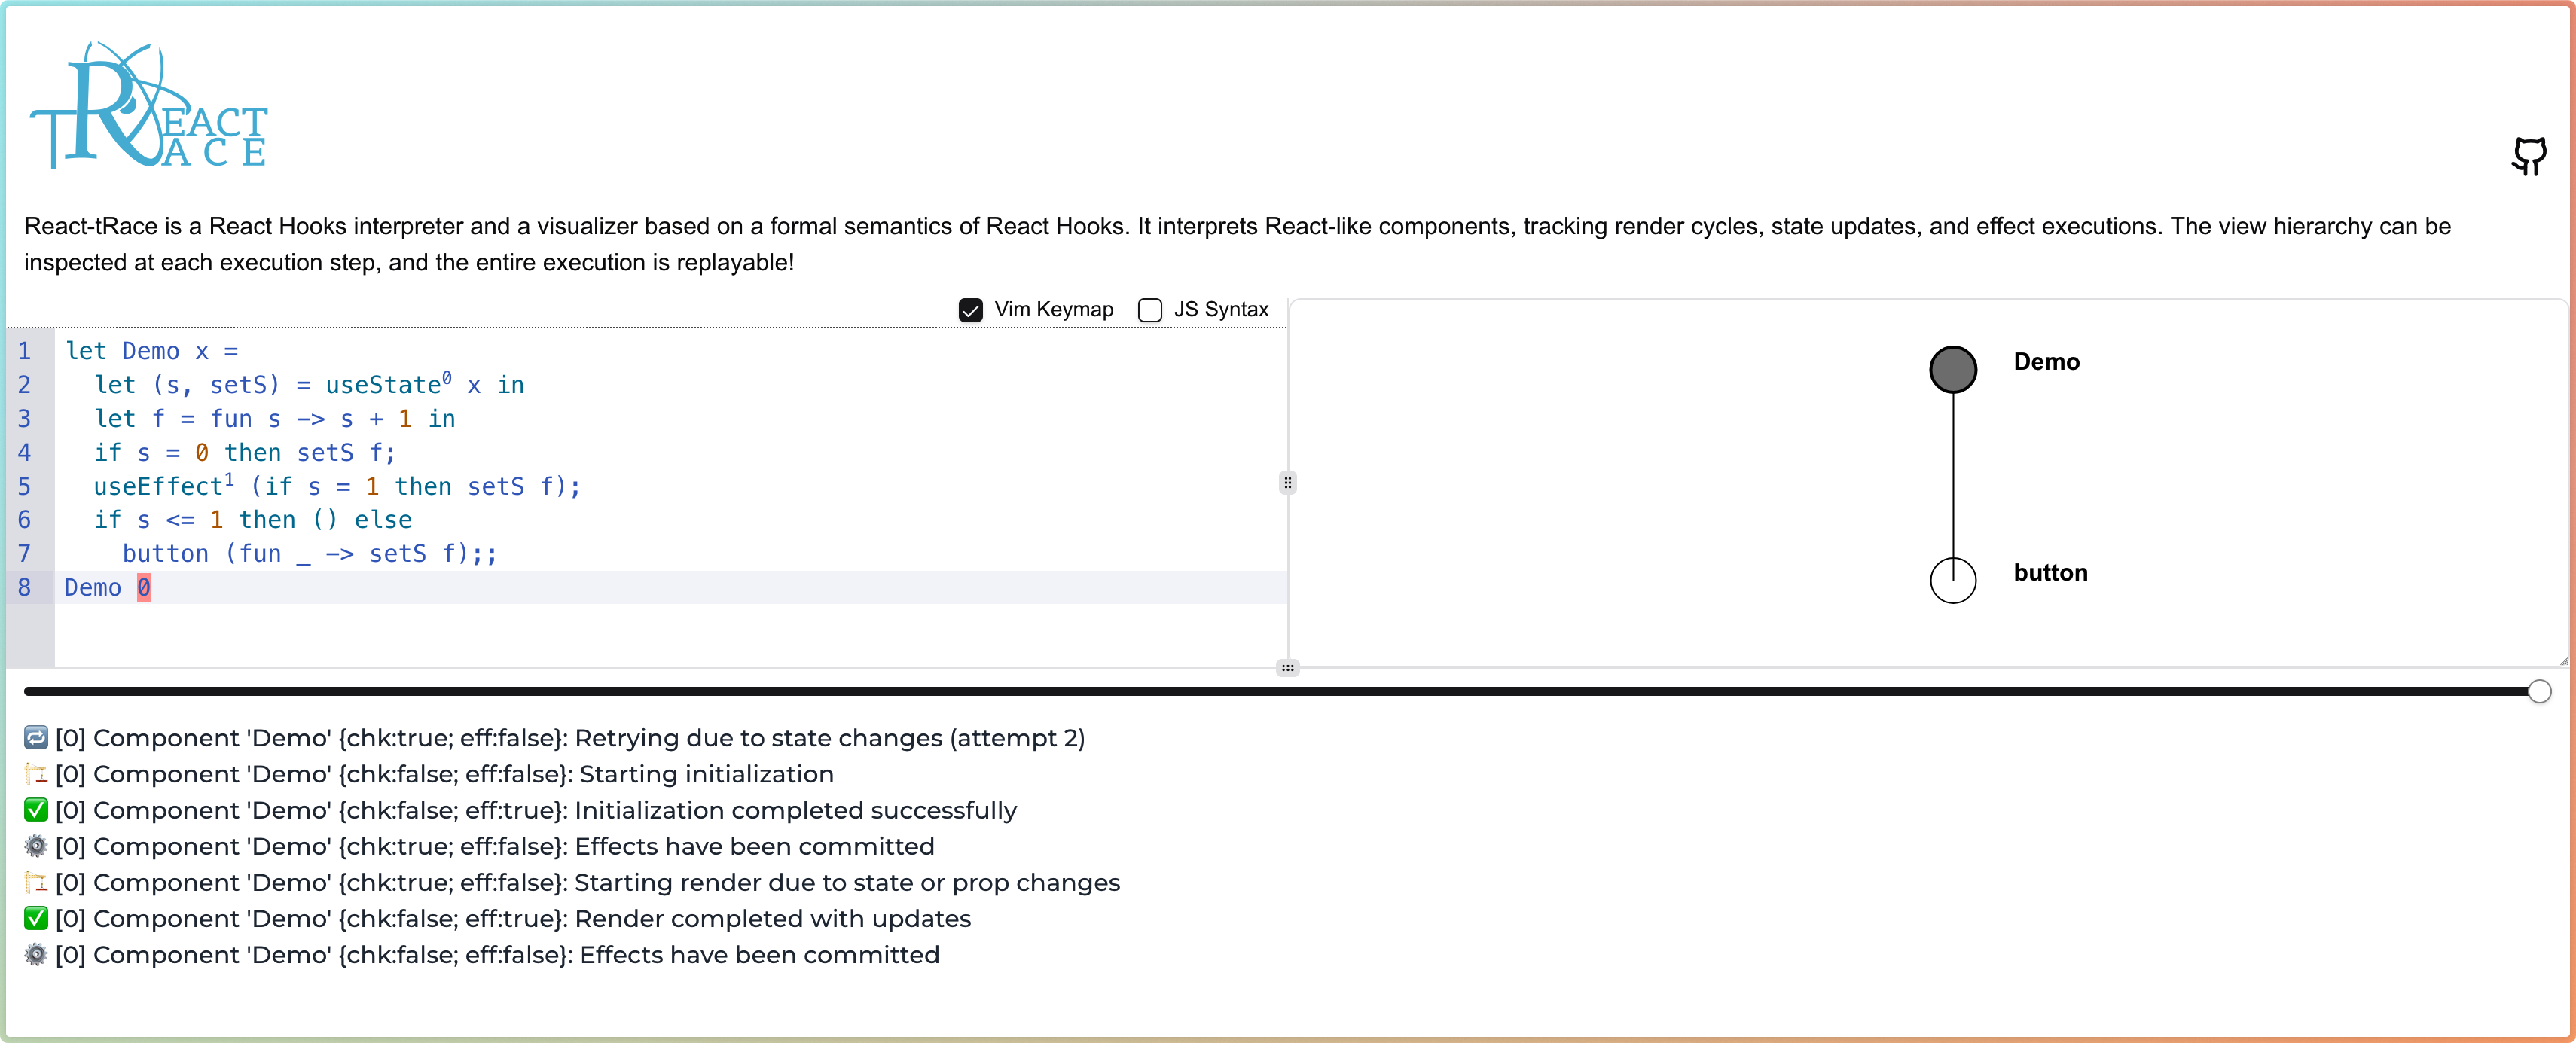
\includegraphics[width=\textwidth]{images/react-trace.png}
  \caption{The \Rtrace{} interpreter and visualizer interface, showing the illustrative example from~\cref{sec:example}.}\label{fig:vis}
\end{figure}

We have implemented a definitional interpreter and a visualization tool (\cref{fig:vis}) to help developers understand the behavior of React Hooks, based on the semantics of React Hooks~(\cref{chap:sem}).

The visualizer enables React programmers to examine their programs in an interactive manner:
\begin{itemize}
  \item The view hierarchy can be inspected by visualizing the tree memory.
  \item The execution of the program is explained, automating the step-by-step reasoning in~\cref{sec:example}.
  \item The entire execution is replayable using a slider, allowing thorough examination of re-rendering bugs described in~\cref{chap:pit}.
\end{itemize}

While our visualizer is fully functional and readily usable, we are actively developing additional features to enhance its capabilities.
Planned or in-progress enhancements include more comprehensive state and trace visualization, experimental JS translation to bridge the gap between real-world React applications, and a direct preview of the rendered UI.
% Our tool demonstrates how semantics-oriented approaches can produce practical developer utilities.

\paragraph{Implementation} The \Rtrace{} interpreter is a faithful implementation of our semantics written in OCaml~5, with the visualization front-end implemented using React with ReScript (\href{https://rescript-lang.org/}{rescript-lang.org}) and TypeScript (\href{https://www.typescriptlang.org/}{typescriptlang.org}).
We used the Js\_of\_ocaml compiler \citep{VouBal14Bytecode} to emit JS code that interfaces with our front-end.

% It is noteworthy to mention that effect handlers in OCaml~5.3 \citep{SivDolWhiKelJafMad21Retrofitting} were used to model computations as an alternative to a monadic interpreter.
% For instance, scoped contexts such as~$m, \delta, \sigma, \pi$ for semantic functions shown in \cref{fig:dependencies} are implemented using effect handlers \citep{Pre15Introduction}.
% Operations on the environment, tree memory, view, definition table, etc. are done by performing effects, which are then handled by the installed deep effect handlers.
% Using effects helped us to flexibly add components in our semantics, enabling rapid prototyping.

The source code is available at \href{https://github.com/Zeta611/react-trace}{\gh{Zeta611/react-trace}}, and the visualizer interface can be accessed online at \href{https://react-trace.vercel.app/}{\nolinkurl{react-trace.vercel.app}}.
